\newpage
\section{Attacks symmetrical algs in smart cards}

\subsection{Differential Power Analysis} 
\label{Differential_Power_Analysis}

Differential Power Analysis was originally proposed by P.Kocher, 
J.Jaffe and B.June \cite{crypto-1999-kocher} in 1998.
As the power consumption is dependant from value manipulated by the algorithm 
-see section ~\ref{To model power consumption}-
this dependency can leads to an attack when a manipulated value depends only on
few bits of the secret key.

The principle of the Differential Power Analysis is to make hypothesis about those a
part of the key, to simulate the power consumption under this hypothesis and then
to perform statistical 
-see section ~\ref{Presentation of different statistical methods}-
comparisons with real curves. 

This attack require a large number of power trace, comparing to Simple Power Analysis,
but it can reveal the secret key of a device even if the recorded power traces are extremely 
noisy.
This dependency can be exploited when a variable is manipulated and only depend on few bits
of the secret key.\\
To achieve such an analysis several hypothesis have to be made:

\begin{itemize}
	\item  about the model of power consumption, this is very sensitive.
	\item  about the way that the algorithm is designed.
	\item  about the manipulated variable.
	\item  about a part of the key, noted $K_j$, on which depend the targeted variable.
\end{itemize}


Taking the example of the DES algorithm, the aim of this attack is
to reveal round key, for that it calculate 8 part of the round key, 
in order to get all the key with it. 
Once the attack is achieved, it can be launched again to calculate another part of the 
round key, and finally get the whole round key.
\vspace{3mm}

\underline{\textbf{Step 1}}: Choosing an Intermediate Result.

The first thing to do is to choose an intermediate result of the algorithm that is executed by
the attacked device, by example on the DES algorithm we can choose the output of a S-box.

So to attack an algorithm with this method you need an exemplary of this one, 
please note that we are only
interested in the value of this intermediate result so the type of 
implementation of the target algorithm
does not matter, only its design does(\textit{e.g.} where we take the intermediate value don't depend 
od the Des implementation).

This intermediate result have to be a function $f(d,k)$, called \textit{selection function},
where $k$ is a small part of the key and, most of the time, $d$ is either the plain-text
 or the cypher-text.To avoid false peaks the result of the $ f $ function must be uniformly distributed : 
\begin{center}
\textit{i.e.}  $\forall k\; \mathbb{P}(f(M_j, K_k)=1) = \frac{1}{2}$
\end{center}
 \vspace{3mm}
 
\underline{\textbf{Step 2}}: Measuring the Power Consumption.

Here we will simulate a run of the smart card.
To do so we'll need to have several text that is to be a plaintext or a cypher text,
noted $d_i$ $ \in\{ d_1, \ldots,d_D \}$ and to encrypt -or decrypt- all of this values.
For each of these encryptions -or decryptions- runs the attacker will know this value involved in the
calculation of the intermediate result chosen at step 1 and he will records the corresponding power trace.

Each of this trace, $\mathcal{C}_i$, will be noticed as following $(t_{i,j})_j=( t_{i,1}, \ldots , t_{i,T})$
for the $i^{th}$  consumption trace corresponding to $d_i$ and where $T$ is denotes the length of the trace.
The attacker measure the trace for each data block, and hence, the traces can be written as
matrix $\mathcal{T}$ of size $D \times T$.
 
It is important for DPA attacks that the measured trace are correctly aligned, because this means that
the power consumption value of each column of $\mathcal{T}$ need to be caused by the same operation. 
In order to do this two different means: to record traces on a oscilloscope with trigger signal, 
or to align curve with mathematical algorithms.


\newpage
\underline{\textbf{Step 3}}: Calculating Hypothetical Intermediate Values.

The next step of the attack is to calculate hypothetical intermediate value for every possible 
choice of $k_j$. Let's write $k_j  \in \{ k_1, \ldots, k_K \} $ where $K$ denotes the total number
of possible choice for the round key. $K$ will be 64 bits because the length of one round key is 6
bytes and for each byte there are only two possibilities $1$ or $0$. In the context of DPA
attacks, we usually refer to those elements as \textit{key hypothesis}.
Now an attacker can easily calculate $f(d_i,k_j)$.
This construction results in a matrix $\mathcal{V}$ of size $D \times K$ defined by the
following relation:
\begin{center}
$\forall (i,\;j)$ such as $1\leq i \leq D$ and $1 \leq j \leq K: v_{i,j}= f(d_i,k_j)$
\end{center}

The $j^{th}$ column of $\mathcal{V}$ contains the intermediate results that have been calculated on the key
hypothesis $k=k_j$ and as we are trying all possibility for $k$ the value used in the device is one of them.
The goal of DPA is to find this correspondence.
\vspace{3mm}

\underline{\textbf{Step 4}}: Mapping Intermediate Values to Power Consumption Values.

For this purpose, the attacker uses a technique simulation. 
The quality of this simulation strongly depends
on the knowledge of the attacker about the device. \textbf{The better this simulation 
of the attacker matches the
actual power consumption characteristics of the device, the more effective is the DPA attack.} 
We will see next how to do it. This mapping applied to the matrix 
$\mathcal{V}$ give a matrix, noticed $\mathcal{H}$ 
of the same size: $D \times K$.
\vspace{3mm}

\underline{\textbf{Step 5}}: Comparing Hypothetical to Recorded Consumption. 

Now the final step of the DPA attack can be performed:
each column of the matrix $\mathcal{H}$ is compared 
with each column of the matrix $\mathcal{T}$ with some
statistical method. This means that the attacker compares 
the Hypothetical power consumption values
of each key hypothesis with the recorded trace at every position.
The result of this comparison is a matrix $\mathcal{R}$ of size  $K \times T$,
 where each element $r_{i,j}$
contains the result of the comparison between the columns 
$h_{i}$ and $t_{j}$. The comparison is done based
on algorithms I will discuss later. \textbf{But in every algorithm, 
one thing is similar : the value $r_{i,j}$ is the
higher, the better the columns $h_{i}$ and $t_{j}$ match.} 
The key of the attacked device can hence be
revealed based on the following observation.\\
\indent The power traces correspond to the power consumption 
of the device while it executes a
cryptographic algorithm using different data inputs. 
The intermediate result that has been chosen in
\textbf{step 1} is a part of this algorithm. 
That's why the device needs to calculate the intermediate
values of the matrix $\mathcal{V}$ during the execution of the algorithm.
Consequently, also the recorded traces depend on these intermediate
values at some position.\\
\indent The hypothetical power consumption values
 in $\mathcal{H}$ have been simulated by the attacker
based on the values of the matrix $\mathcal{V}$. 
In  fact, the column of $\mathcal{H}$ and $\mathcal{T}$ are strongly related and
lead to the highest values in the matrix $\mathcal{R}$. 
All other values of $\mathcal{R}$ are low because
the other columns of  $\mathcal{H}$ and $\mathcal{T}$ are not strongly related.\\
\textbf{ The index of the line in which is the highest values of the matrix $\mathcal{R}$ is
reveals which of the key hypothesis is the more probable.}

\underline{\textbf{\textit{problem 1}}} In practice the matrix $\mathcal{R}$ 
have sometimes the same
coefficient. In this case, the attacker has usually not measured enough power traces to estimate
the relationship between the columns of  $\mathcal{H}$ and $\mathcal{T}$.
Indeed the more traces an attacker measures, the more elements 
are in the columns $\mathcal{H}$ and
 $\mathcal{T}$, and more precisely the attacker can determine the relationship between the columns.

\underline{\textbf{\textit{problem 2}}} This also implies that the more measurements are made,
the smaller relationships between the columns can be determined. 
So I had to get a good number of
measurements. On a DES implementation with no counter measure 5000 traces are 
enough to find a round key, see section ~\ref{Copy of the first attack report}.

The following diagram is illustrating the steps 3 to 5 of a DPA attack.
\newpage
\vspace{2cm}
\begin{center}
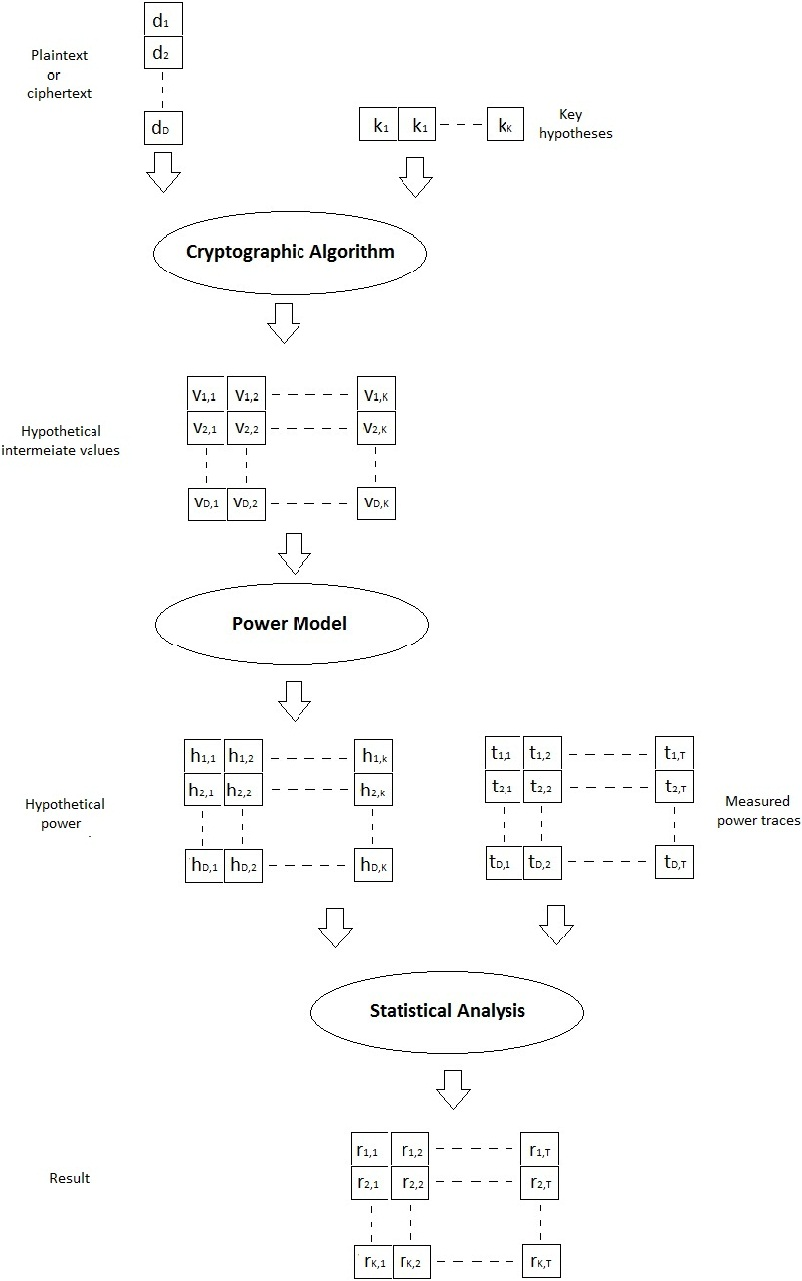
\includegraphics[width=140mm,height=185mm]{images/diagramCPA.jpg}\\
\textit{Figure 16. Schema of the DPA attack}
\end{center}

\newpage
\subsection{About the power model}
\label{About_the_power_model}

\paragraph*{}Once the $\mathcal{V}$ matrix is filled, 
it have to be transformed to $\mathcal{H}$ matrix
thanks to power consumption model, this model is crucial 
because it will depend the success of the attack.

\paragraph*{Linear models}

This model is simple and efficient because it permit to separate the consumption of 
the target electrical component (register, RAM cell, bus ) from the rest of the circuit.

For every component and at any time we have :
\begin{center}
$C =  C_{\mathit{all \; the \; circuit \; but \; the \; component}}+C_{component}$
\end{center}
Nowadays, technology CMOS is most widespread to implement the integrated circuits.
With this kind of technology, as said in \cite{phd-Messerges-2000}, the component mainly consumes
current when there is a change of state of the logical parts between two blows of clock:
the static consumption is negligible.

\paragraph*{Asymmetric model}
Let $ B = (\beta_m,...,\beta_1) $ the value that will be saved in the targeted component,
and $ A = (\alpha_m,...,\alpha_1) $ the value previously stored in this component.\\
Let also $ c_{01}^i$ and $ c_{10}^i$ be respectively the amount of currents needed to
change a bit from 0 to 1 and from 1 to 0 for the $i^{th}$ bit.
If after a clock the value of the register is set to $ B $, the consumption after the shot clock is:
\begin{center}
$C(t) = \theta+  \sum\limits_{i=1}^{m} (1-\alpha_i)\beta_i c_{01} + \alpha_i(1-\beta_i)c_{10} $
\end{center}
where $\theta$ is the electrical consumption due to others part of the circuit, and 
$ c_{01} ,\;\;c_{10}$ and $\theta$ are function of time.

\paragraph*{Symmetric models}
As proposed by Brier \cite{eprint-2003-brier} we assume that $ c_{01} = c_{10}$,
the model of power consumption, can be simplified using 
 $ d_{\mathcal{H}} $ for the Hamming distance operator to: 
\begin{center}
$C(t) = \theta(t)  + d_{\mathcal{H}}(A,B) \times c(t) $
\end{center}
where $ d_{\mathcal{H}} $ is the Hamming distance operator.\\
This model can be simplified again if assumed that the reference state A is always zero,
this model has been proposed by T.Messerges, where $ \omega_{\mathcal{H}} $ is the Hamming weight operator.
\begin{center}
$C(t) = \theta(t)  + \omega_{\mathcal{H}}(B) \times c(t)  $
\end{center}


\paragraph*{Hamming weight}
Finally the most common, for the -realistic- case that $\theta $ and $c$ are not considered as function of time:
\begin{center}
$C(t) = \omega_{\mathcal{H}}(B)   $
\end{center}
Other model exist, like the one from S.Aumonier
\nocite{ecrypt-2007} \cite{ecrypt-2007-aumonier} based on the concept of mutual
information. This model is much more general and precise that previous one, 
but on the other hand this model is much more slower.



\paragraph*{Conclusions}
\begin{itemize}
\item There are a many power model more or less close to the reality.
As always, the simpler it is, the quicker it is and of course the less precise it is.
\item Note that on Kocher's original article \cite{crypto-1999-kocher}: "mono-bit DPA"
the intermediate value is only constituted of one bit and the present section who
studied the problem of the power consumption is not relevant in this case.

\end{itemize}


